\documentclass{standalone}
\usepackage{tikz}
\usetikzlibrary{patterns, positioning}

\begin{document}
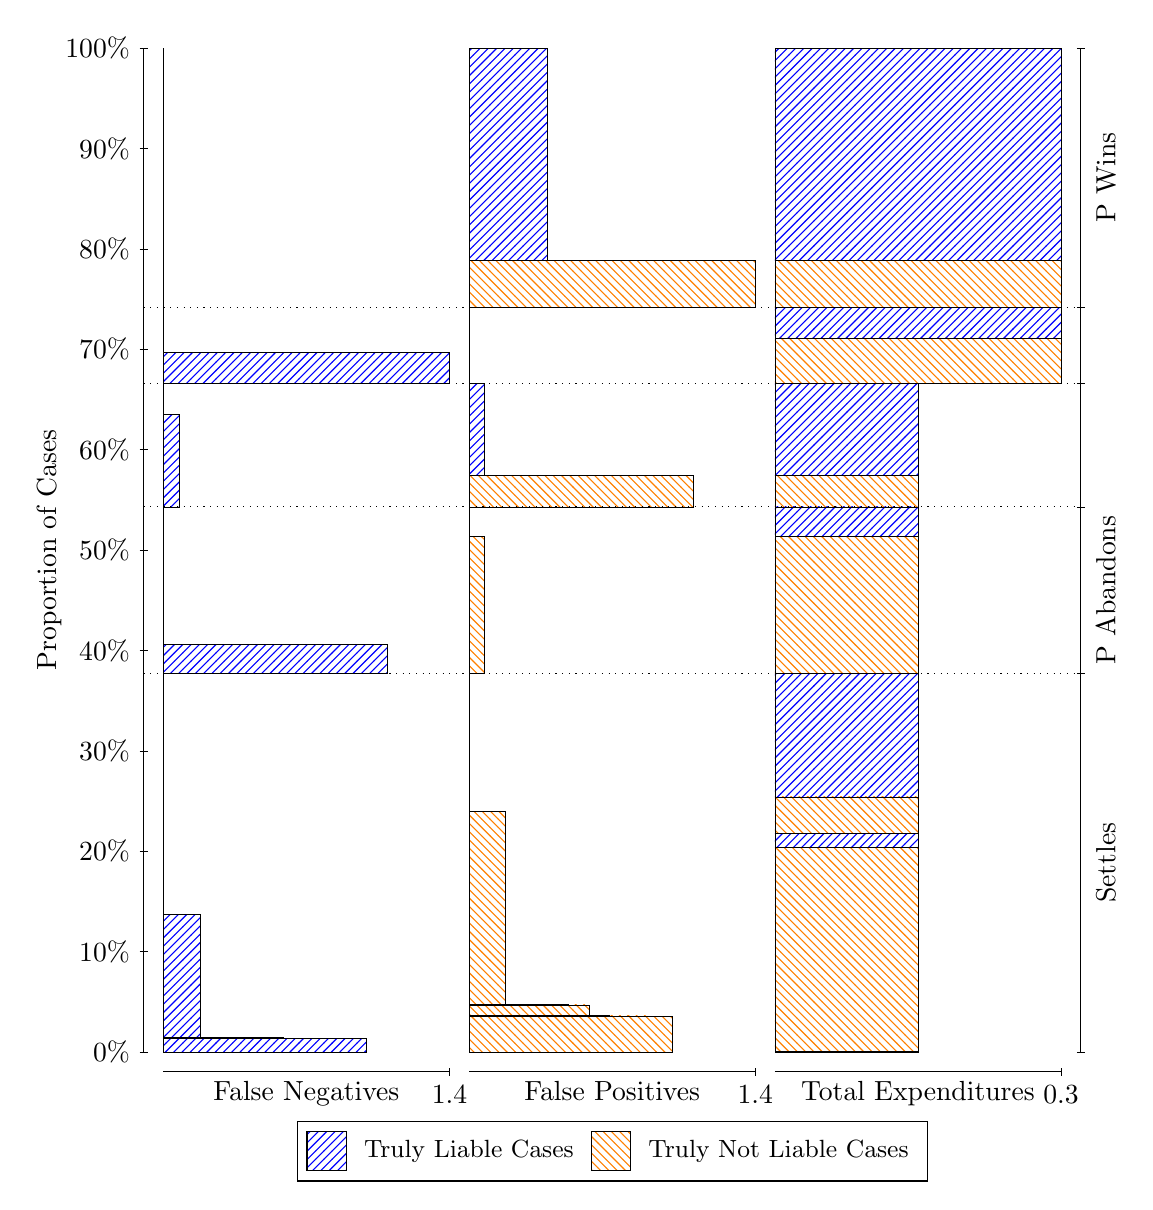
\begin{tikzpicture}
\draw[black, very thin] (1.5,1.75) -- (1.5,14.5);
\node[rotate=90, anchor=center] at (0.3, 8.125) {Proportion of Cases};
\draw[black, very thin] (1.45,1.75) -- (1.55,1.75);
\node[anchor=east] at (1.45, 1.75) {0\%};
\draw[black, very thin] (1.45,3.025) -- (1.55,3.025);
\node[anchor=east] at (1.45, 3.025) {10\%};
\draw[black, very thin] (1.45,4.3) -- (1.55,4.3);
\node[anchor=east] at (1.45, 4.3) {20\%};
\draw[black, very thin] (1.45,5.575) -- (1.55,5.575);
\node[anchor=east] at (1.45, 5.575) {30\%};
\draw[black, very thin] (1.45,6.85) -- (1.55,6.85);
\node[anchor=east] at (1.45, 6.85) {40\%};
\draw[black, very thin] (1.45,8.125) -- (1.55,8.125);
\node[anchor=east] at (1.45, 8.125) {50\%};
\draw[black, very thin] (1.45,9.4) -- (1.55,9.4);
\node[anchor=east] at (1.45, 9.4) {60\%};
\draw[black, very thin] (1.45,10.675) -- (1.55,10.675);
\node[anchor=east] at (1.45, 10.675) {70\%};
\draw[black, very thin] (1.45,11.95) -- (1.55,11.95);
\node[anchor=east] at (1.45, 11.95) {80\%};
\draw[black, very thin] (1.45,13.225) -- (1.55,13.225);
\node[anchor=east] at (1.45, 13.225) {90\%};
\draw[black, very thin] (1.45,14.5) -- (1.55,14.5);
\node[anchor=east] at (1.45, 14.5) {100\%};

\draw[black, very thin] (13.4,1.75) -- (13.4,14.5);
\draw[black, very thin] (13.35,1.75) -- (13.45,1.75);
\node[anchor=west] at (13.35, 1.75) {};
\draw[black, very thin] (13.35,6.5565) -- (13.45,6.5565);
\node[anchor=west] at (13.35, 6.5565) {};
\draw[black, very thin] (13.35,8.6729) -- (13.45,8.6729);
\node[anchor=west] at (13.35, 8.6729) {};
\draw[black, very thin] (13.35,10.245) -- (13.45,10.245);
\node[anchor=west] at (13.35, 10.245) {};
\draw[black, very thin] (13.35,11.208) -- (13.45,11.208);
\node[anchor=west] at (13.35, 11.208) {};
\draw[black, very thin] (13.35,14.5) -- (13.45,14.5);
\node[anchor=west] at (13.35, 14.5) {};

\draw[black, very thin, pattern color=blue, pattern=north east lines] (1.75,1.75) rectangle (4.3264,1.9183);
\draw[black, very thin, pattern color=blue, pattern=north east lines] (1.75,1.9183) rectangle (4.0621,1.9184);
\draw[black, very thin, pattern color=blue, pattern=north east lines] (1.75,1.9184) rectangle (3.7979,1.9186);
\draw[black, very thin, pattern color=blue, pattern=north east lines] (1.75,1.9186) rectangle (3.5336,1.9188);
\draw[black, very thin, pattern color=blue, pattern=north east lines] (1.75,1.9188) rectangle (3.2694,1.9316);
\draw[black, very thin, pattern color=blue, pattern=north east lines] (1.75,1.9316) rectangle (3.0052,1.9317);
\draw[black, very thin, pattern color=blue, pattern=north east lines] (1.75,1.9317) rectangle (2.7409,1.9319);
\draw[black, very thin, pattern color=blue, pattern=north east lines] (1.75,1.9319) rectangle (2.4767,1.932);
\draw[black, very thin, pattern color=blue, pattern=north east lines] (1.75,1.932) rectangle (2.2124,3.4978);
\draw[black, very thin, pattern color=orange, pattern=north west lines] (1.75,3.4978) rectangle (1.75,6.5565);
\draw[black, very thin, pattern color=blue, pattern=north east lines] (1.75,6.5565) rectangle (4.5906,6.9277);
\draw[black, very thin, pattern color=orange, pattern=north west lines] (1.75,6.9277) rectangle (1.75,8.6729);
\draw[black, very thin, pattern color=blue, pattern=north east lines] (1.75,8.6729) rectangle (1.9482,9.8466);
\draw[black, very thin, pattern color=orange, pattern=north west lines] (1.75,9.8466) rectangle (1.75,10.245);
\draw[black, very thin, pattern color=blue, pattern=north east lines] (1.75,10.245) rectangle (5.3833,10.633);
\draw[black, very thin, pattern color=orange, pattern=north west lines] (1.75,10.633) rectangle (1.75,11.208);
\draw[black, very thin, pattern color=orange, pattern=north west lines] (1.75,11.208) rectangle (1.75,11.806);
\draw[black, very thin, pattern color=blue, pattern=north east lines] (1.75,11.806) rectangle (1.75,14.5);
\draw[black, very thin, pattern color=orange, pattern=north west lines] (5.6333,1.75) rectangle (8.2097,2.2069);
\draw[black, very thin, pattern color=orange, pattern=north west lines] (5.6333,2.2069) rectangle (7.9455,2.2082);
\draw[black, very thin, pattern color=orange, pattern=north west lines] (5.6333,2.2082) rectangle (7.6812,2.2095);
\draw[black, very thin, pattern color=orange, pattern=north west lines] (5.6333,2.2095) rectangle (7.417,2.2108);
\draw[black, very thin, pattern color=orange, pattern=north west lines] (5.6333,2.2108) rectangle (7.1527,2.3486);
\draw[black, very thin, pattern color=orange, pattern=north west lines] (5.6333,2.3486) rectangle (6.8885,2.3487);
\draw[black, very thin, pattern color=orange, pattern=north west lines] (5.6333,2.3487) rectangle (6.8885,2.3506);
\draw[black, very thin, pattern color=orange, pattern=north west lines] (5.6333,2.3506) rectangle (6.6242,2.3524);
\draw[black, very thin, pattern color=orange, pattern=north west lines] (5.6333,2.3524) rectangle (6.36,2.3541);
\draw[black, very thin, pattern color=orange, pattern=north west lines] (5.6333,2.3541) rectangle (6.0958,4.8087);
\draw[black, very thin, pattern color=blue, pattern=north east lines] (5.6333,4.8087) rectangle (5.6333,6.5565);
\draw[black, very thin, pattern color=orange, pattern=north west lines] (5.6333,6.5565) rectangle (5.8315,8.3017);
\draw[black, very thin, pattern color=blue, pattern=north east lines] (5.6333,8.3017) rectangle (5.6333,8.6729);
\draw[black, very thin, pattern color=orange, pattern=north west lines] (5.6333,8.6729) rectangle (8.4739,9.0713);
\draw[black, very thin, pattern color=blue, pattern=north east lines] (5.6333,9.0713) rectangle (5.8315,10.245);
\draw[black, very thin, pattern color=orange, pattern=north west lines] (5.6333,10.245) rectangle (5.6333,10.819);
\draw[black, very thin, pattern color=blue, pattern=north east lines] (5.6333,10.819) rectangle (5.6333,11.208);
\draw[black, very thin, pattern color=orange, pattern=north west lines] (5.6333,11.208) rectangle (9.2667,11.806);
\draw[black, very thin, pattern color=blue, pattern=north east lines] (5.6333,11.806) rectangle (6.6242,14.5);
\draw[black, very thin, pattern color=orange, pattern=north west lines] (9.5167,1.75) rectangle (11.333,1.7554);
\draw[black, very thin, pattern color=blue, pattern=north east lines] (9.5167,1.7554) rectangle (11.333,1.7559);
\draw[black, very thin, pattern color=orange, pattern=north west lines] (9.5167,1.7559) rectangle (11.333,4.3485);
\draw[black, very thin, pattern color=blue, pattern=north east lines] (9.5167,4.3485) rectangle (11.333,4.5296);
\draw[black, very thin, pattern color=orange, pattern=north west lines] (9.5167,4.5296) rectangle (11.333,4.9904);
\draw[black, very thin, pattern color=blue, pattern=north east lines] (9.5167,4.9904) rectangle (11.333,6.5565);
\draw[black, very thin, pattern color=orange, pattern=north west lines] (9.5167,6.5565) rectangle (11.333,8.3017);
\draw[black, very thin, pattern color=blue, pattern=north east lines] (9.5167,8.3017) rectangle (11.333,8.6729);
\draw[black, very thin, pattern color=orange, pattern=north west lines] (9.5167,8.6729) rectangle (11.333,9.0713);
\draw[black, very thin, pattern color=blue, pattern=north east lines] (9.5167,9.0713) rectangle (11.333,10.245);
\draw[black, very thin, pattern color=orange, pattern=north west lines] (9.5167,10.245) rectangle (13.15,10.819);
\draw[black, very thin, pattern color=blue, pattern=north east lines] (9.5167,10.819) rectangle (13.15,11.208);
\draw[black, very thin, pattern color=orange, pattern=north west lines] (9.5167,11.208) rectangle (13.15,11.806);
\draw[black, very thin, pattern color=blue, pattern=north east lines] (9.5167,11.806) rectangle (13.15,14.5);
\draw[black, dotted] (1.5,6.5565) -- (13.4,6.5565);
\draw[black, dotted] (1.5,8.6729) -- (13.4,8.6729);
\draw[black, dotted] (1.5,10.245) -- (13.4,10.245);
\draw[black, dotted] (1.5,11.208) -- (13.4,11.208);
\draw[black, very thin] (1.75,1.5) -- (5.3833,1.5);
\node[anchor=north] at (3.5667, 1.5) {False Negatives};
\draw[black, very thin] (5.3833,1.45) -- (5.3833,1.55);
\node[anchor=north] at (5.3833, 1.45) {1.4};

\draw[black, very thin] (5.6333,1.5) -- (9.2667,1.5);
\node[anchor=north] at (7.45, 1.5) {False Positives};
\draw[black, very thin] (9.2667,1.45) -- (9.2667,1.55);
\node[anchor=north] at (9.2667, 1.45) {1.4};

\draw[black, very thin] (9.5167,1.5) -- (13.15,1.5);
\node[anchor=north] at (11.333, 1.5) {Total Expenditures};
\draw[black, very thin] (13.15,1.45) -- (13.15,1.55);
\node[anchor=north] at (13.15, 1.45) {0.3};

\node[black, centered, rotate=90] at (13.72, 4.1533) {Settles};
\node[black, centered, rotate=90] at (13.72, 7.6147) {P Abandons};


\node[black, centered, rotate=90] at (13.72, 12.854) {P Wins};

\draw (7.449999999999999,1.5) node[draw=none] (baseCoordinate) {};
\begin{scope}[align=center]
        \matrix[scale=0.5, draw=black, below=0.5cm of baseCoordinate, nodes={draw}, column sep=0.1cm]{
            \node[rectangle, draw, minimum width=0.5cm, minimum height=0.5cm, pattern=north east lines, pattern color=blue] {}; &
            \node[draw=none, font=\small] (B) {Truly Liable Cases}; &
            \node[rectangle, draw, minimum width=0.5cm, minimum height=0.5cm, pattern=north west lines, pattern color=orange] {}; &
            \node[draw=none, font=\small] (B) {Truly Not Liable Cases}; \\
            };
\end{scope}

\end{tikzpicture}
\end{document}